\documentclass[letterpaper, 10 pt, conference]{article} 
\usepackage[english]{babel}
\usepackage{amsmath,amssymb,amscd,amsthm} % variety of useful math macros
\usepackage[inner=1.5 cm, outer = 1.5 cm, top=1 cm, bottom = 1.5 cm]{geometry}
\usepackage{subcaption}
%For inserting graphics
\usepackage{graphicx}
\usepackage[dvipsnames]{xcolor}
\usepackage{listings}
\usepackage[utf8]{inputenc}
\usepackage{hyperref}
\usepackage{array, multirow}
\usepackage{lipsum}
\usepackage{natbib}

\bibliographystyle{abbrvnat}

\newtheorem{thm}{Theorem}
\newtheorem{prop}{Proposition}
\newtheorem{lemma}{Lemma}

\newcommand\A{\ensuremath{\mathbb{A}}}
\newcommand\C{\ensuremath{\mathbb{C}}}
\newcommand\E{\ensuremath{\mathbb{E}}}
\newcommand\F{\ensuremath{\mathbb{F}}}
\newcommand\I{\ensuremath{\mathbb{I}}}
\newcommand\N{\ensuremath{\mathbb{N}}}
\renewcommand{\P}{\ensuremath{\mathbb{P}}}
\newcommand\Q{\ensuremath{\mathbb{Q}}}
\newcommand\R{\ensuremath{\mathbb{R}}}
\newcommand\Z{\ensuremath{\mathbb{Z}}}
\newcommand\one{\ensuremath{\mathbbm{1}}}

\newcommand\cov{\ensuremath{\mathrm{cov}}}
\newcommand\tst{\ensuremath{\mathrm{test}}}

\title{Bayes' Theorem
}

\hypersetup{
	colorlinks=true,
	linkcolor=blue,
	filecolor=magenta,      
	urlcolor=blue,
	citecolor=MidnightBlue
}

\author{G. Palafox}

\begin{document}
\maketitle

\section{Introduction}
The use of diagnostic tests is widespread in modern medicine. As \citet{clinical_epidemiology} mention in their book, \textit{establishing diagnoses is an imperfect process, resulting in a probability rather than a certainty of being right}. Since decisions are made based on the results of these tests, the correct interpretation of their outcome is important, and probability theory can be used to aid with this understanding.

\section{SARS-CoV-2}
 Currently, a strain of coronavirus (SARS-CoV-2, colloquially known as Covid-19) is causing havoc around the world. Diagnostic tests are being used to fight the pandemic, mainly by requiring quarantine for people who test positive, or allowing less movement restrictions for those who test negative (i.e., not quarantining, permitting travel or entrance to places). Given this, it is essential to have a clear understanding of what test results mean. Bayes' theorem, which can be seen in Theorem \ref{bayes_thm}, can help with these interpretations.
 
 \begin{thm}[Bayes' theorem] \label{bayes_thm}
 	Let $(\Omega, \mathcal{F}, \P)$ be a probability space. Let $\lbrace B_i \rbrace_{i \in \N}$ be a partition of $\Omega$ such that $\P(B_i) > 0$ for each $i$, and let $A$ be any event with positive probability. Then
 	\begin{equation}
 	\P(B_i \mid A) = \frac{\P(A \mid B_i) \P(B_i)}{\sum_{j = 1}^{\infty} \P(A \mid B_j) \P(B_j)}.
 	\end{equation}
 \end{thm}
 
 There are four possible outcomes with any diagnostic test: \textbf{true positive}, where a person with the disease tests positive, \textbf{false positive}, where a person does not have the disease yet tests positive, \textbf{false negative}, where a person with the disease tests negative, and \textbf{true negative}, where a person does not have the disease and tests negative. Additionally, with any test, we associate two measurements of how reliable it is: \textit{specificity}, which is the percentage of true negatives out of healthy people, and \textit{sensitivity}, which is the percentage of true positives among people with the disease. Let us denote by $\pm \tst$ the events of having a positive or negative test, and $\pm \cov$ the events of having or not Covid-19. Using this we can express the sensitivity and specificity of a test as conditional probabilities, namely, 
 \begin{equation}
 	\P( +\tst \mid +\cov) = \text{sensitivity}, \quad \P( -\tst \mid -\cov) = \text{specificity}.
 \end{equation}
If specificity and sensitivity are know, all is left to know is the marginal probability $\P(+\cov)$, and Bayes' theorem can give the probability of having Covid-19 given that a test is positive as 
\begin{equation}
\P( +\cov \mid +\tst) = \frac{ \P(+\tst \mid +\cov)\; \P(+\cov) }{ \P(+\tst \mid +\cov) \; \P(+\cov) + \P(+\tst \mid -\cov) \; \P(-\cov)  }.
\end{equation} 
However, two issues arise. The first one is that in the case of Covid-19, sensitivity and specificity are largely unknown for the widely used PCR test \citep{West_Montori_Sampathkumar_2020}. \citet{pointer} found a sensitivity ranging from 71\% to 98\%, and use a specificity of 95\%. The second issue is the non-trivial calculation of $\P(+\cov)$.  \citet{towards_data_science_covid} and  \cite{significance_bayes} calculate it as the number of confirmed cases divided by the total population.  \citet{stat_bayes} consider half the ratio of positive tests in a given population as an estimate of $\P(+\cov)$. Others \citep{Chan2020, Good2020} vary $\P(+\cov)$, since it can naturally vary depending on who you are testing (random people, people with symptoms, hospital workers, etc.). Personally, the author feels the latter approach gives more insight, since it is adapted easier to different scenarios. 
%\begin{thm}[Total probability theorem]\label{total_prob}
%Let $(\Omega, \mathcal{F}, \P)$ be a probability space. Let $\lbrace B_i \rbrace_{i \in \N}$ be a partition of $\Omega$ such that $\P(B_i) > 0$ for each $i$. Then
%\begin{equation}
%\P(A) = \sum_{i = 1}^{\infty} \P(A \mid B_i) \, \P(B_i).
%\end{equation}
%\end{thm}
\subsection{The case of Nuevo León}
 Consider the case of the Mexican state of Nuevo León. As of October 24, 2020, Nuevo Leon had 77807 confirmed Covid cases in a 5.4 million population \citep{casos_covid_nl, datos_nl}.  If $\P(+\cov)$ is calculated as confirmed cases over population, that would give $\P(+\cov) = 0.0144$.  Assuming a sensitivity of 71\% and specificity of 95\%, this would give 
\begin{equation}	
	\P(+\cov \mid +\tst) = \frac{(.71) (0.0144)}{(.71)(0.0144) + (.05)(.9856)} = 0.17.
\end{equation}

It may seem counter-intuitive that a positive test gives you only a 17\% of having the disease, but this is a consequence of the seemingly low probability of being infected. Consider, on the other hand, that around 40\% of tests performed in Nuevo Leon turn out positive \citep{indicadores_nl}. If we use half of this value as $\P(+\cov)$, Bayes' theorem would give $\P(+\cov \mid +\tst) = 0.78$. As it is seen in Figure \ref{fig:covid}, how widespread the disease is (measured by the marginal probability of being infected) impacts greatly on the interpretation of the test. Specificity and sensitivity, which are not well known for the Covid-19 test, also affect greatly\footnote{The notebook with the code creating these graphics, as well as this report, can be found in the Github Repository: \url{https://github.com/palafox794/AppliedProbabilityModels/tree/master/Assignment8}}. 

\begin{figure}
	\centering
	\begin{subfigure}{0.3\linewidth}
		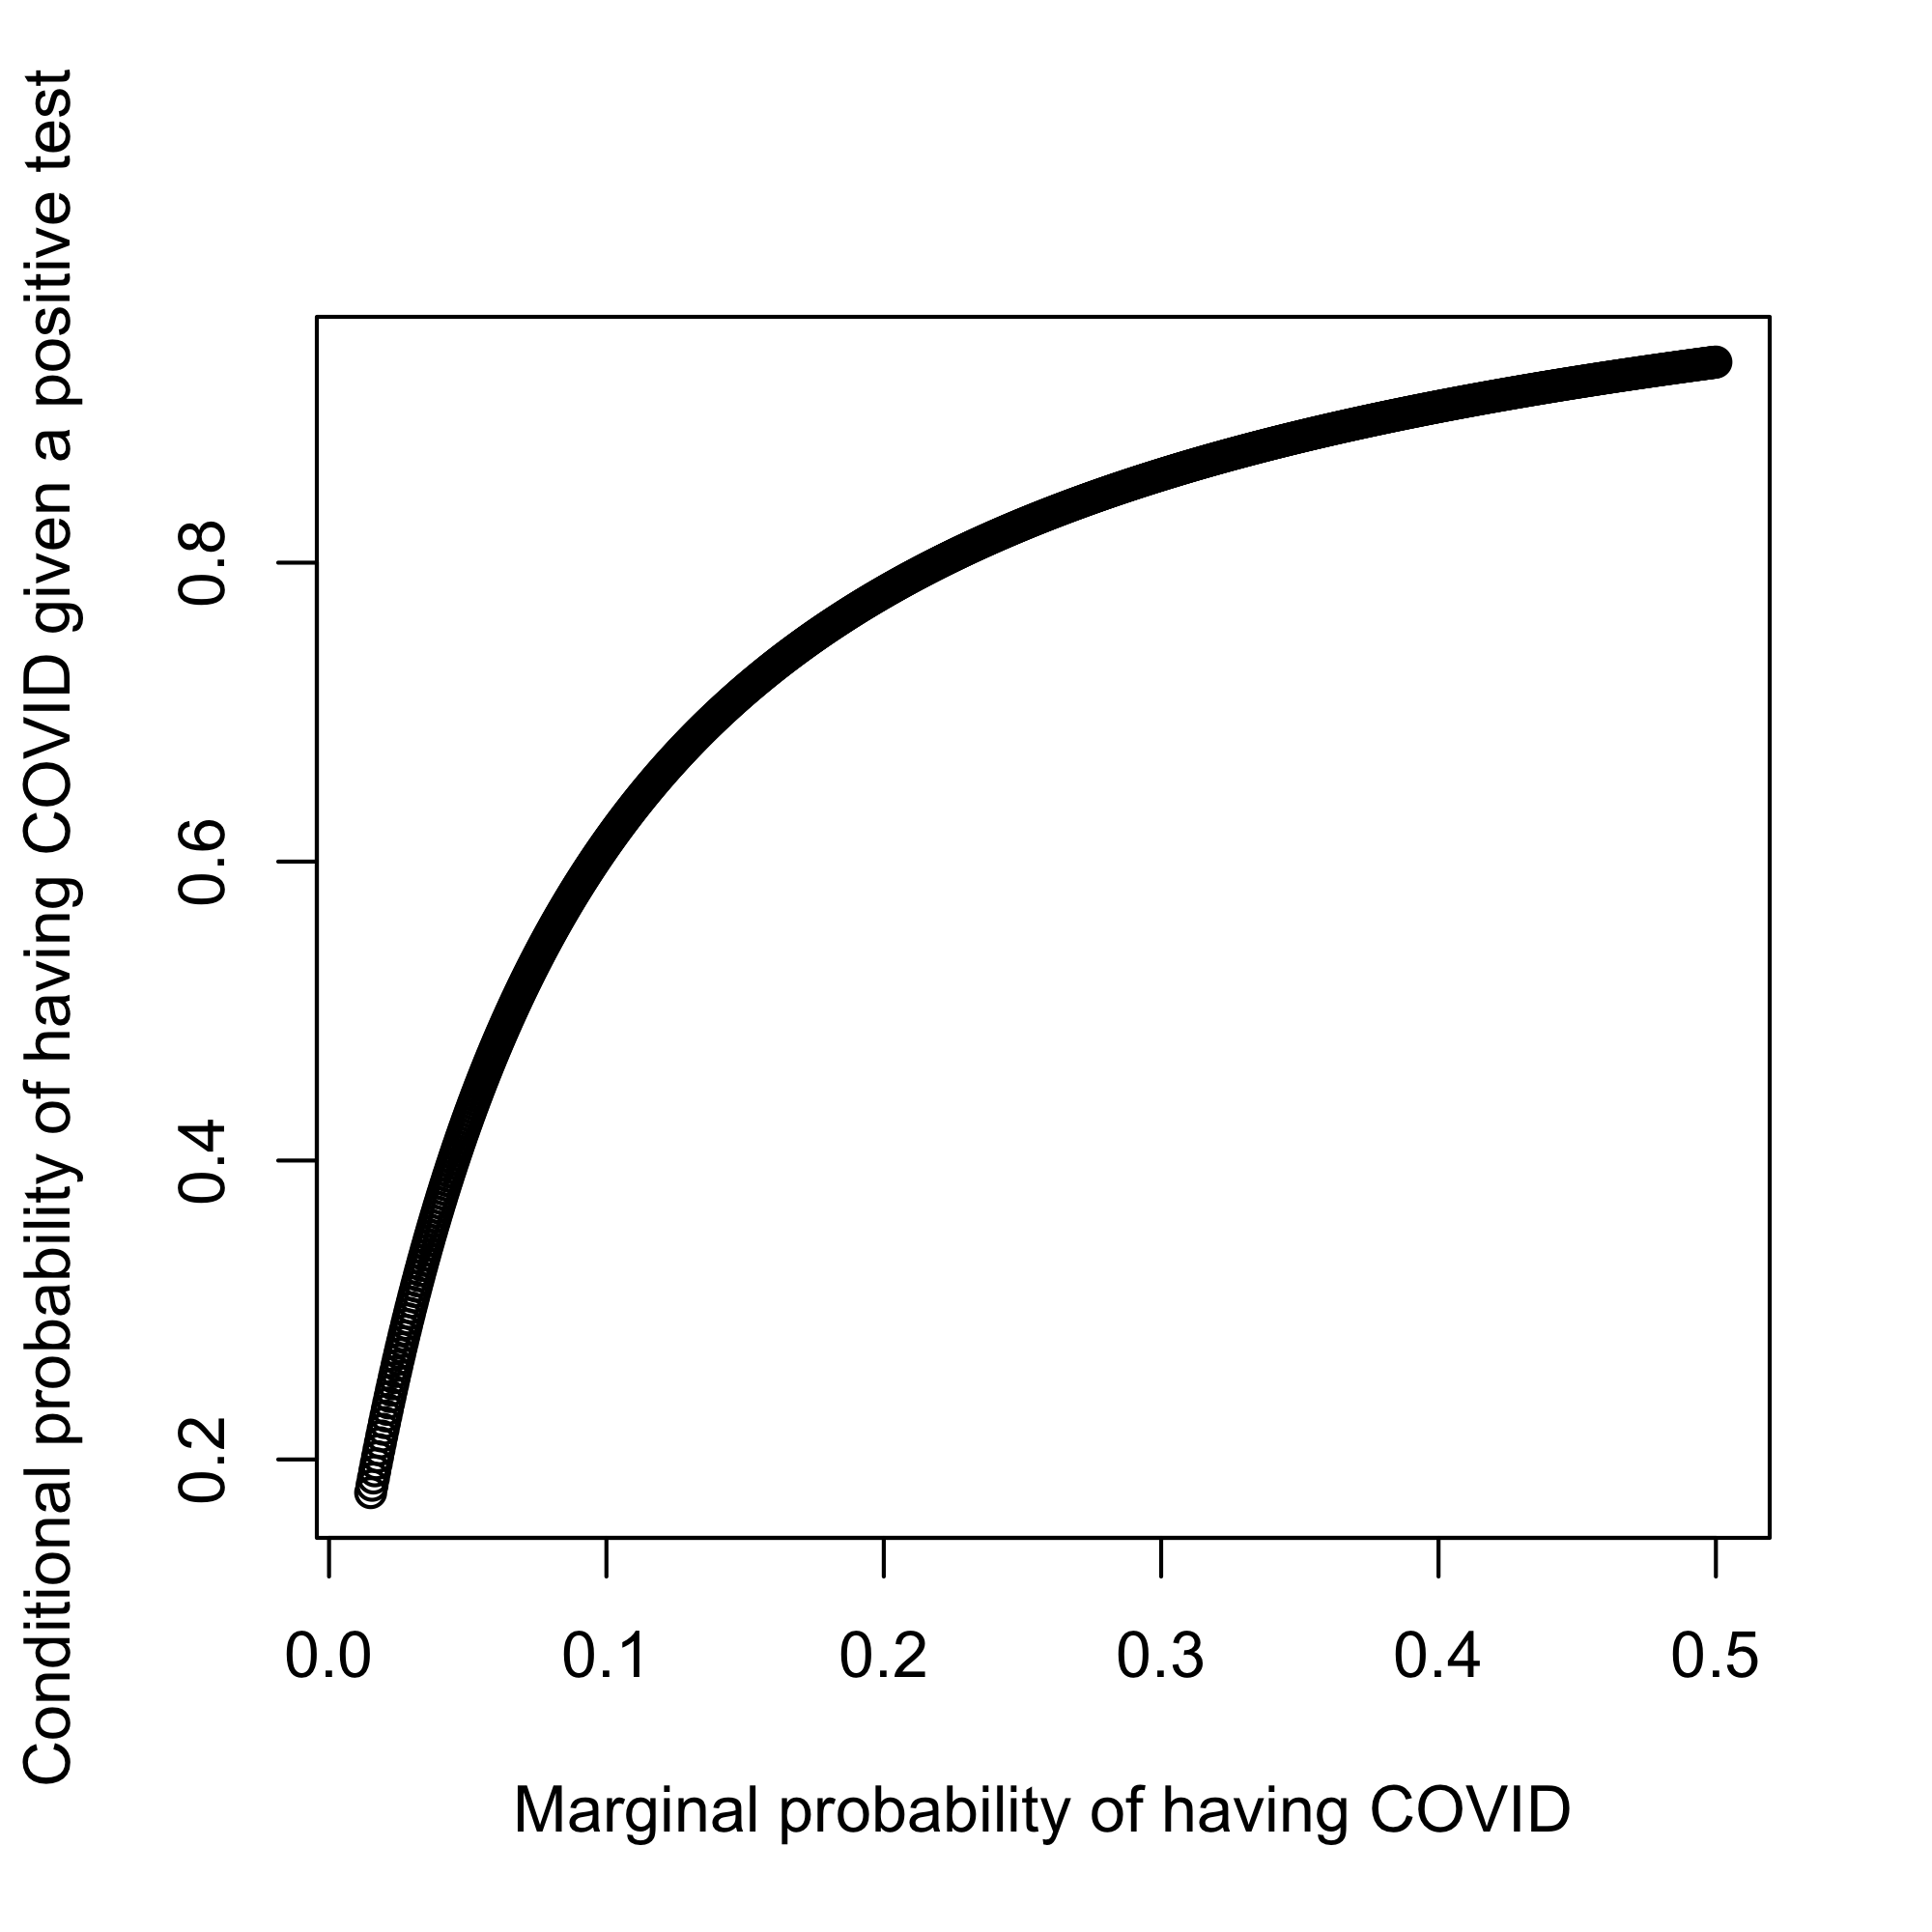
\includegraphics[width=\linewidth]{covid_sens71_spec95}
		\caption{Sensitivity of 71\%, specificity of 95\%.}
		\label{fig:covid_sens71_spec95}
	\end{subfigure}
	\hfill
	\begin{subfigure}{0.3\linewidth}
		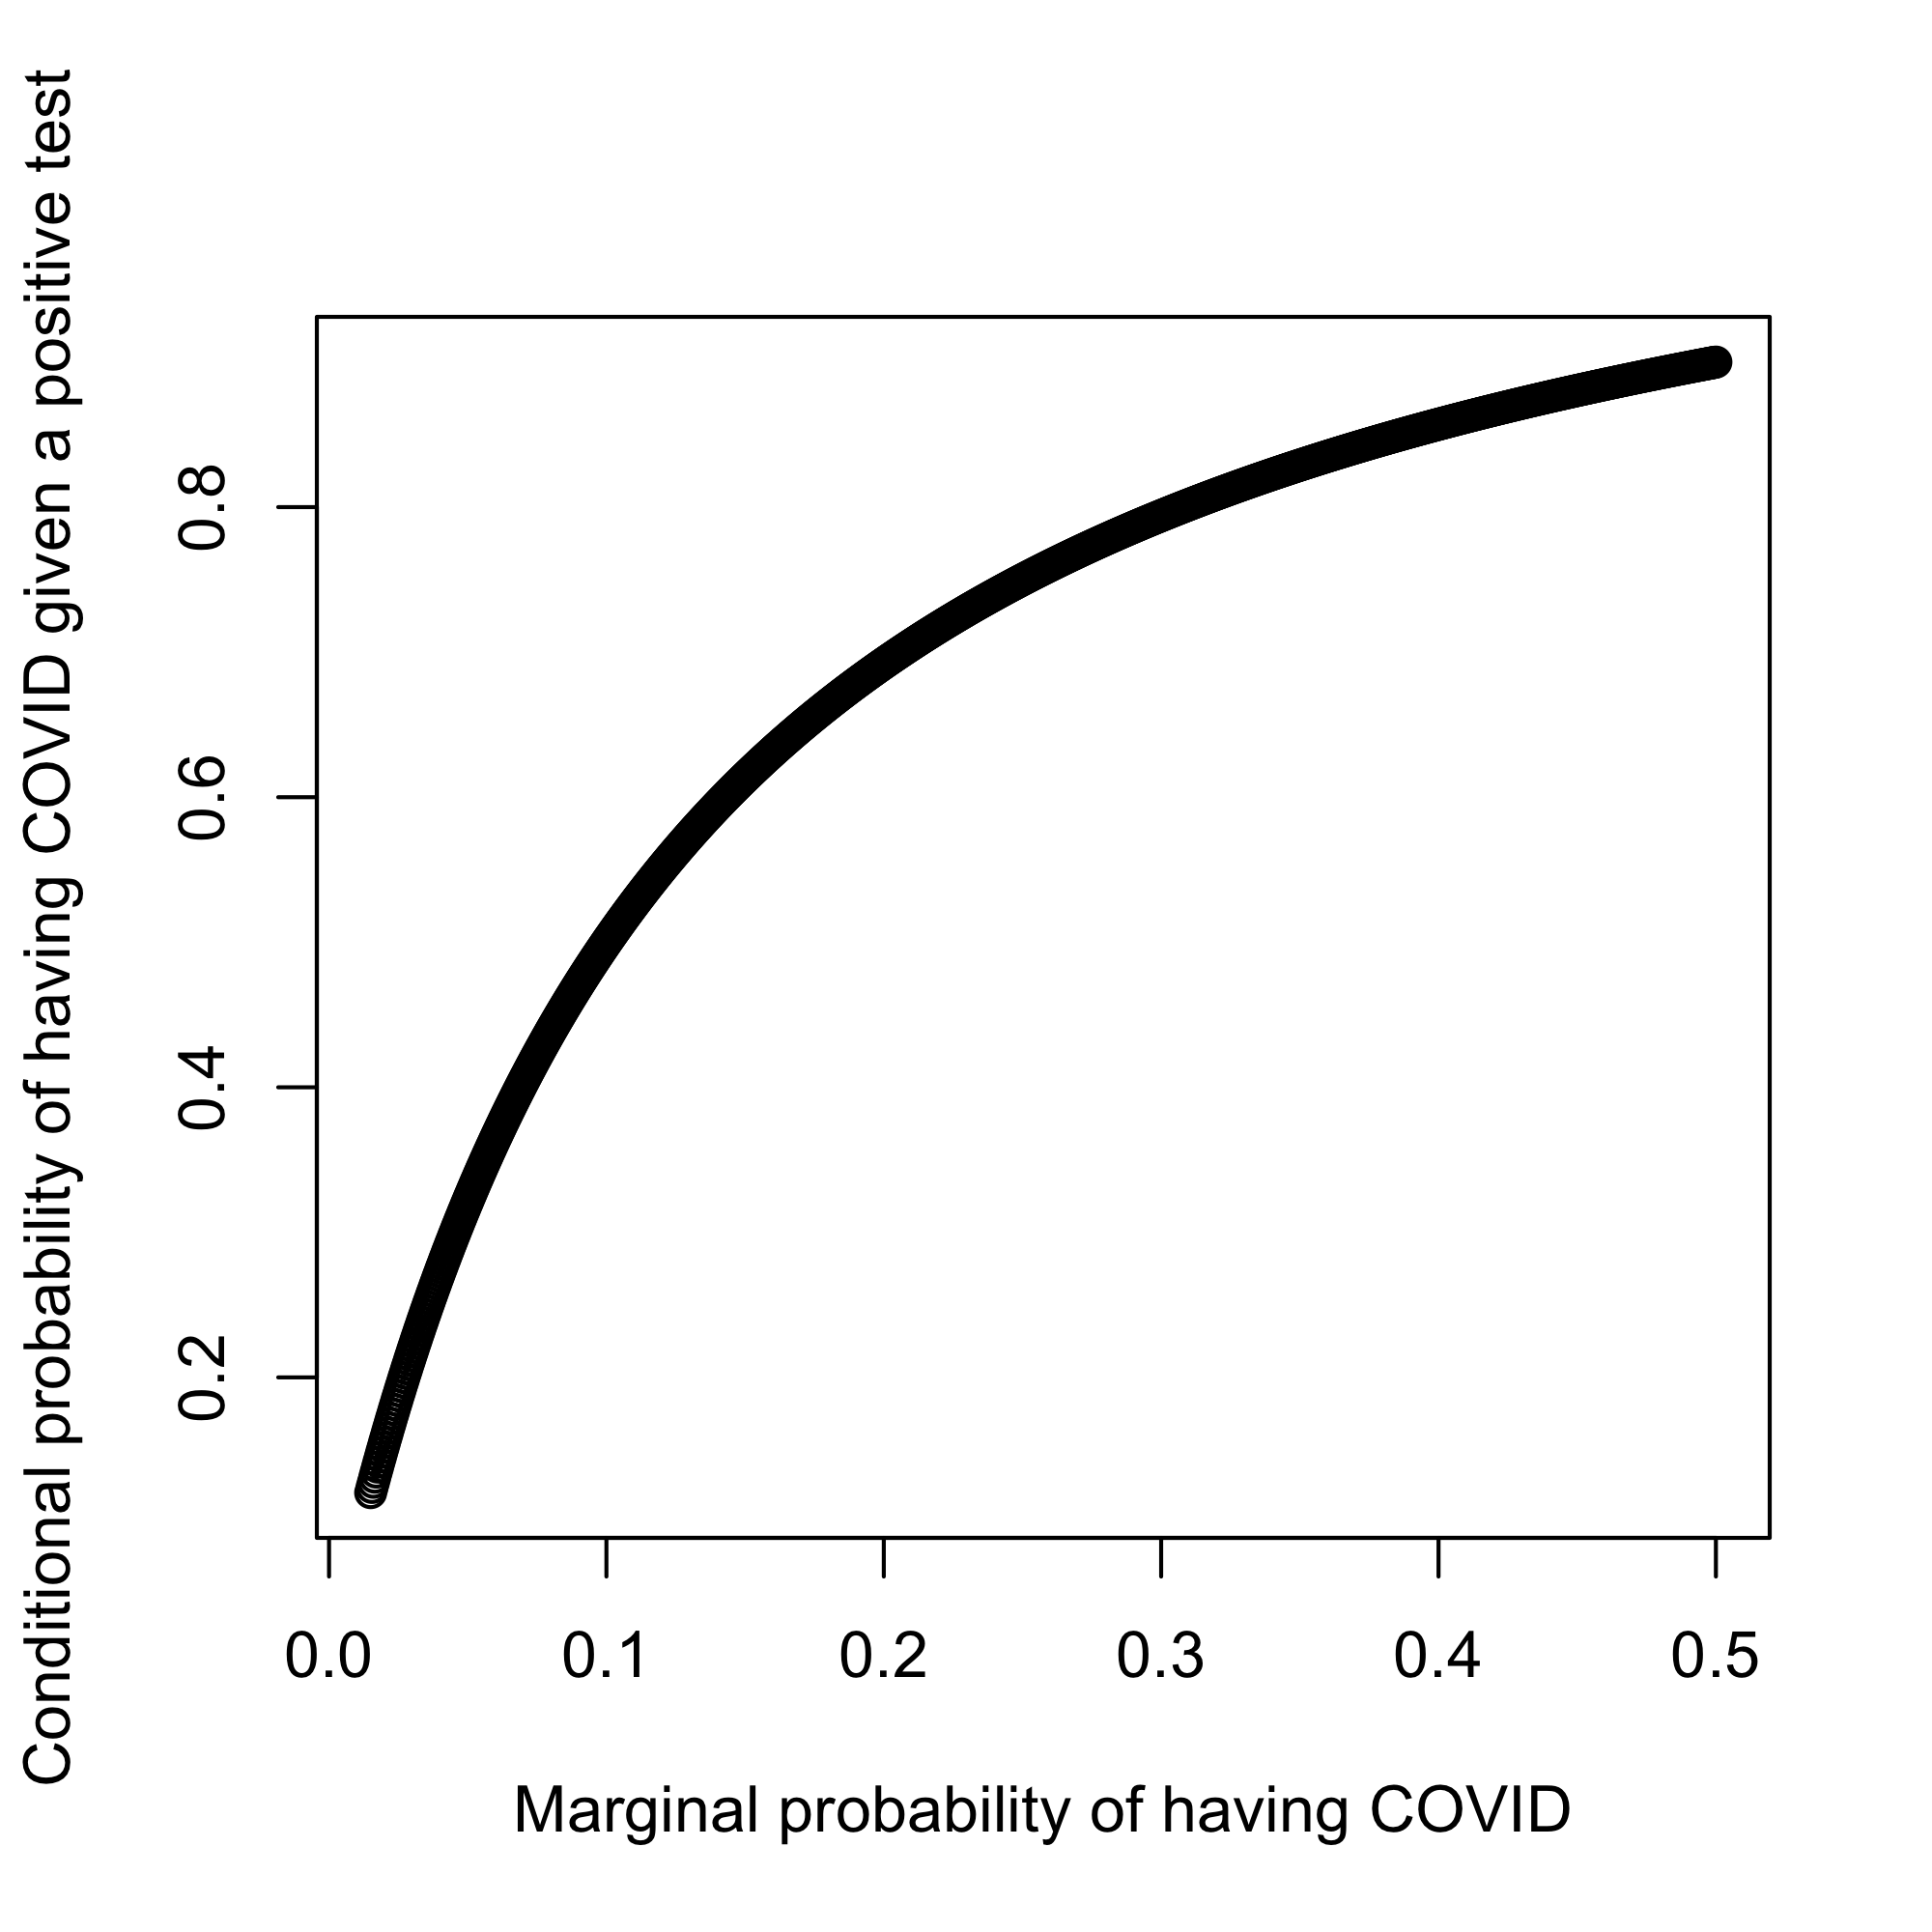
\includegraphics[width=\linewidth]{covid_sens90_spec90}
		\caption{Sensitivity of 90\%, specificity of 90\%.}
		\label{fig:covid_sens90_spec90}
	\end{subfigure}
	\hfill
	\begin{subfigure}{0.3\linewidth}
		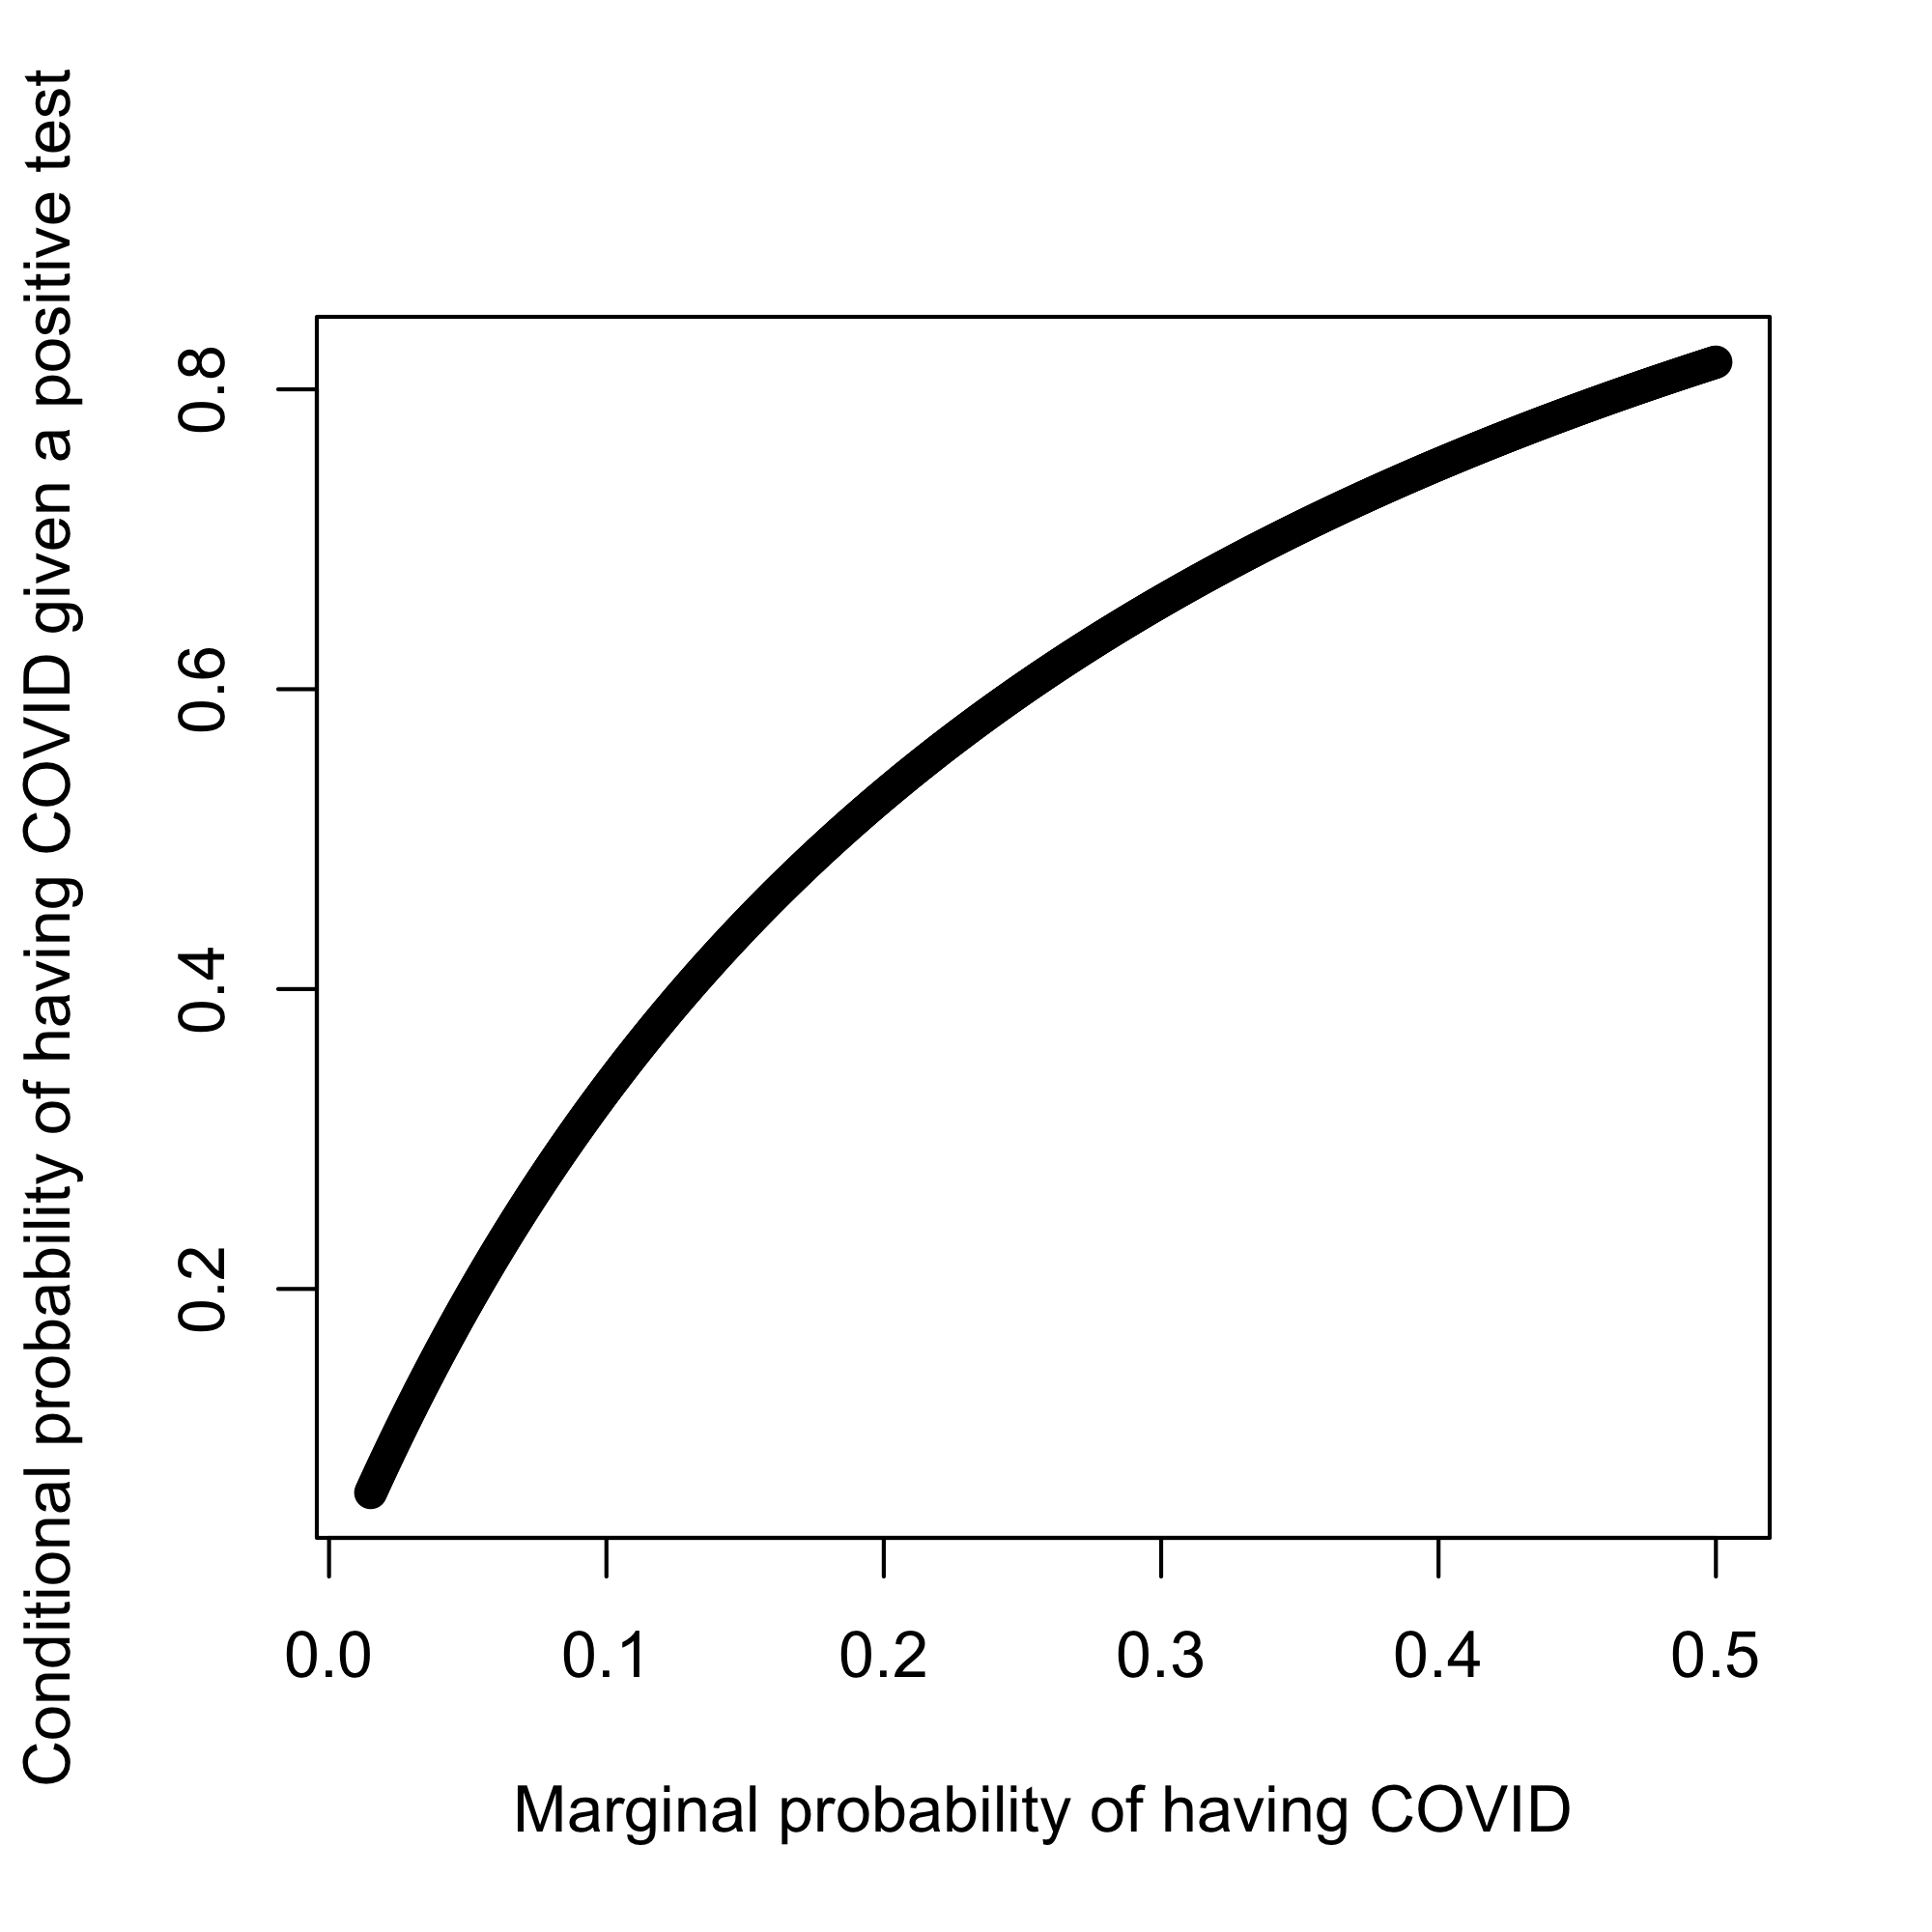
\includegraphics[width=\linewidth]{covid_sens90_spec80}
		\caption{Sensitivity of 90\%, specificity of 80\%.}
		\label{fig:covid_sens90_spec80}
	\end{subfigure}
	\caption{Marginal vs. conditional probability, varying specificity and sensitivity of tests.} 
	\label{fig:covid}
\end{figure}

\section{HIV}
Unlike the tests for the new coronavirus, tests for HIV have a well-established specificity and sensitivity of over 99\% \citep{mmwr_weekly}. Of course, the conditional probability when interpreting a positive result still depends on the prevalence of HIV in the community, i.e., in the marginal probability of being HIV positive. However, this allow us to vary only that parameter, fixing the specificity and sensitivity of the test. For reference, considering $\P(+\mathrm{hiv}) = 1.2 / 327.5 = 0.003$ (cases in the United States over population of the United States, both at the end of 2018 \citep{us_pop_clock, hiv_cdc}), would give $\P(+\mathrm{hiv} \mid +\tst) = 0.78$, using a sensitivity and specificity of 99\%. Varying this marginal probability, with sensitivity and specificity fixed, changes the conditional probability as seen in Figure \ref{fig:hiv}.

\begin{figure}
\centering
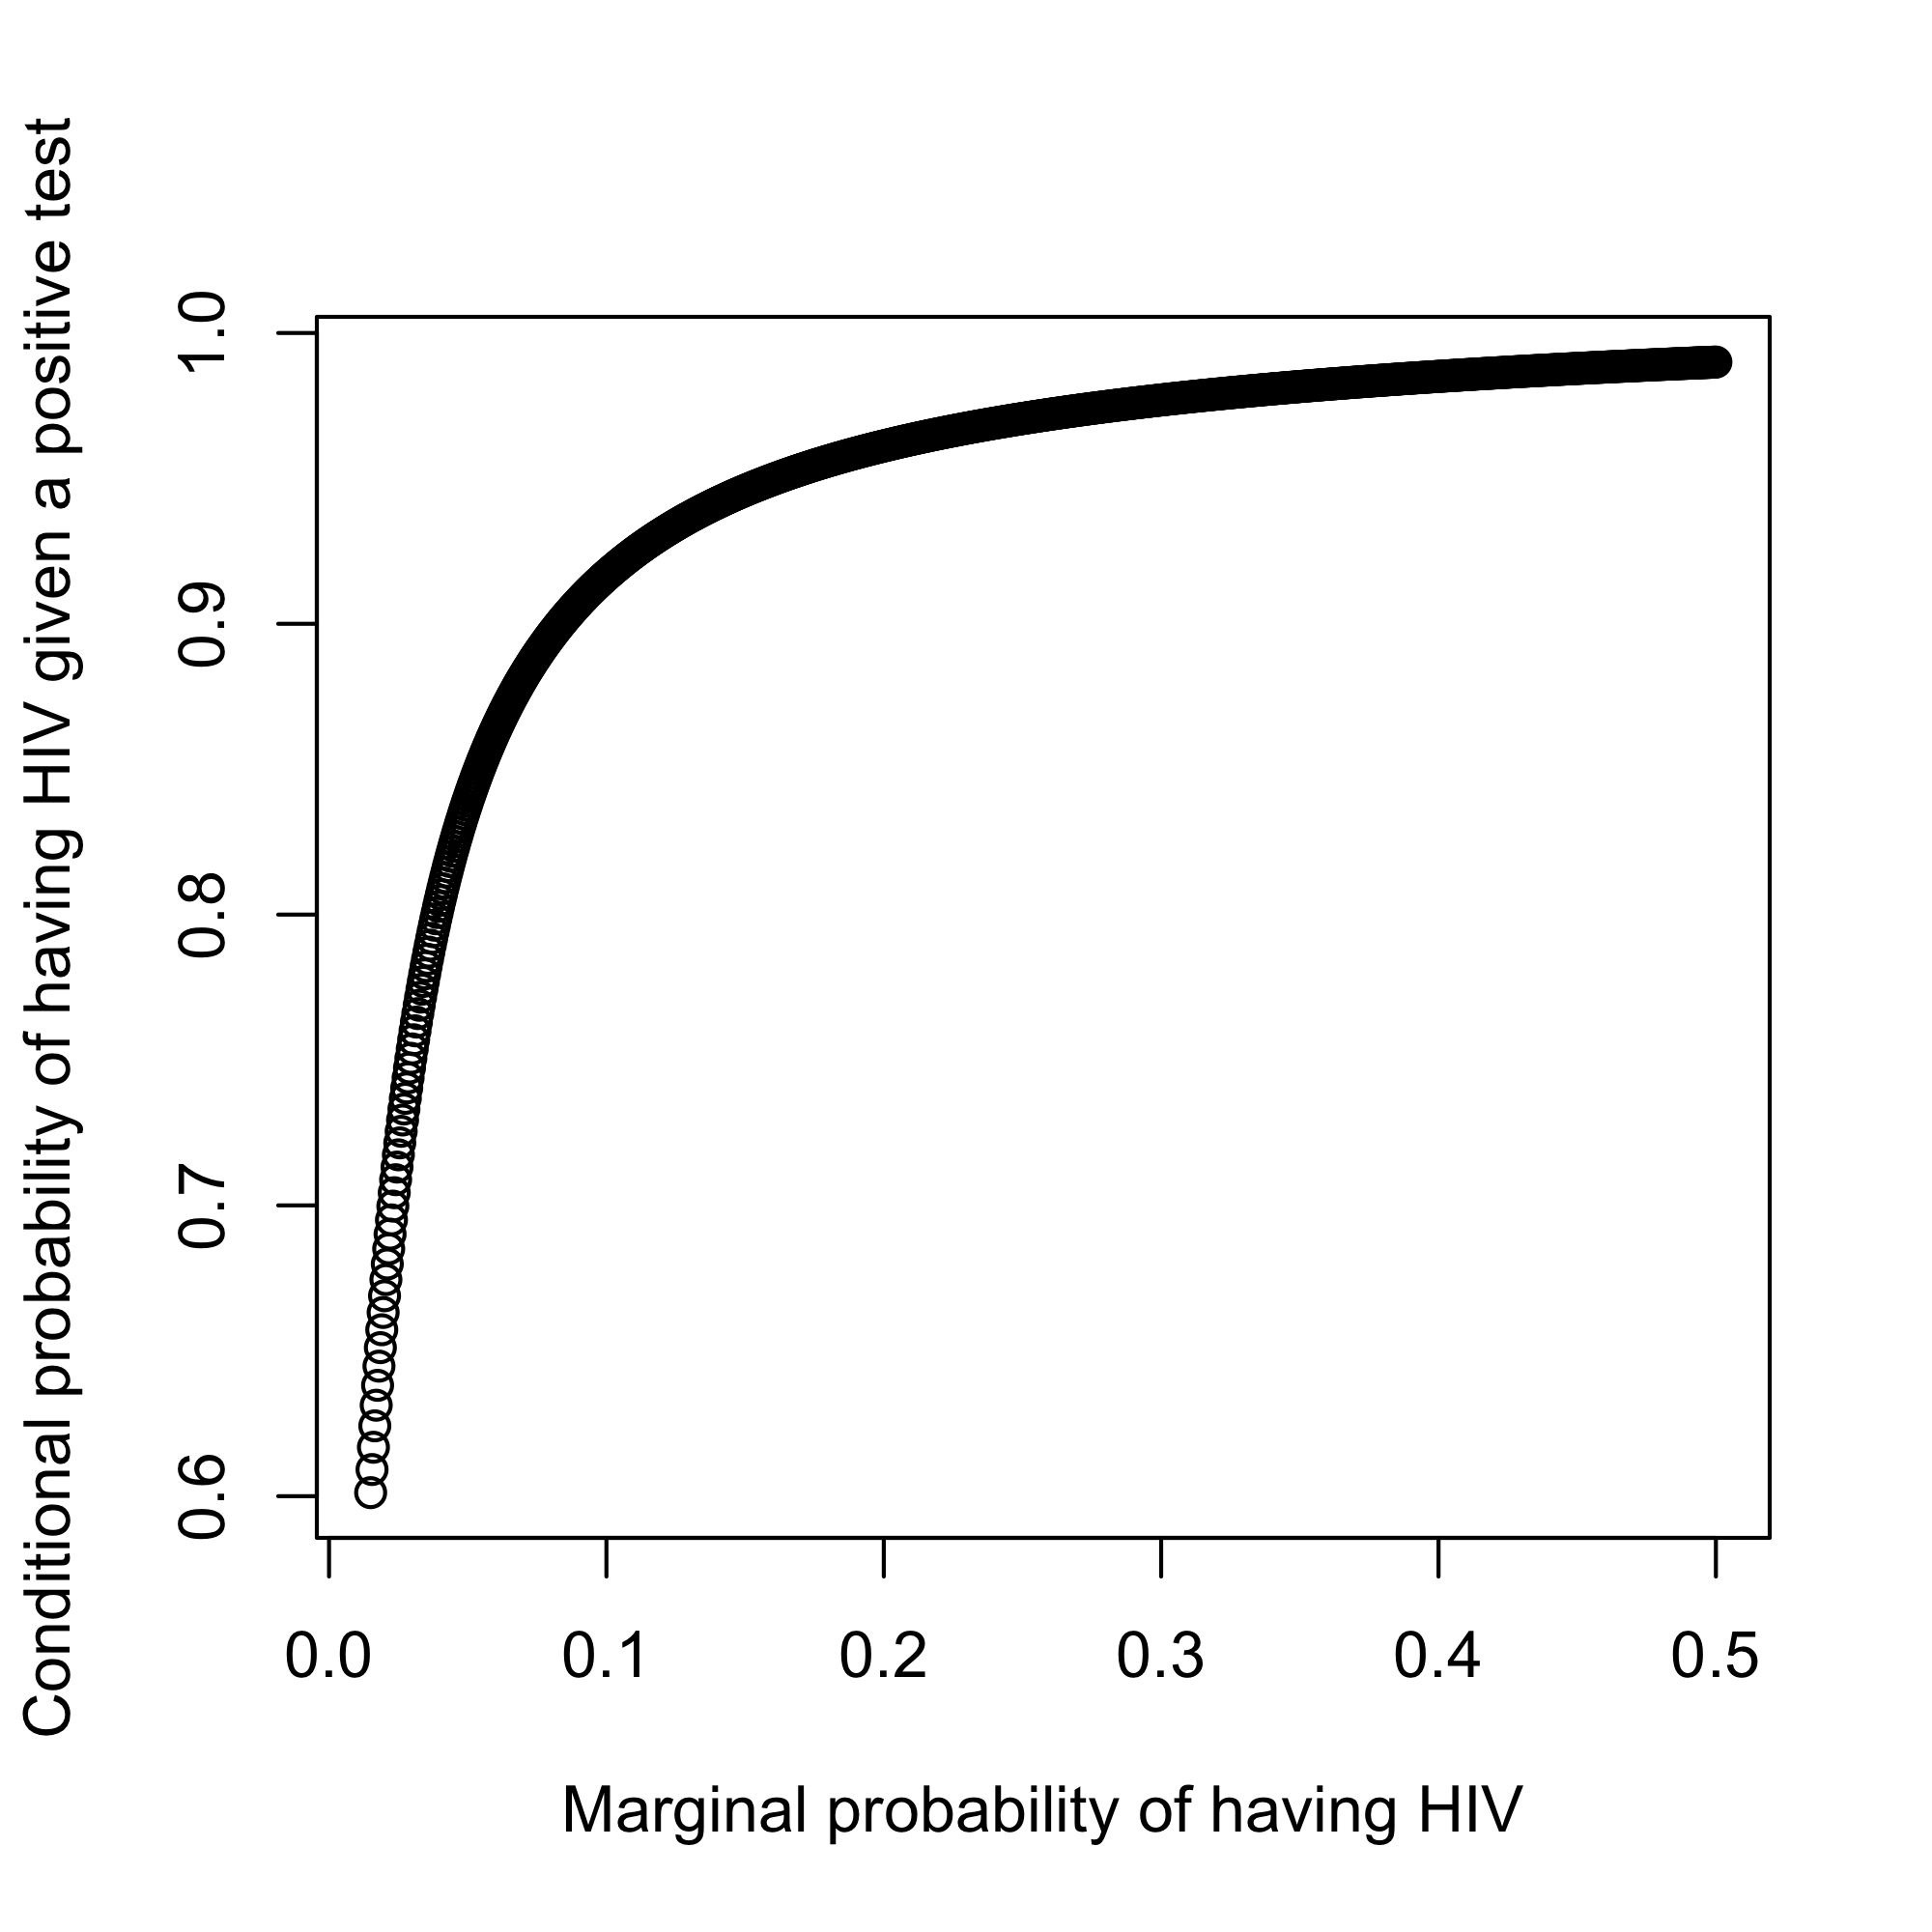
\includegraphics[width=.5\linewidth]{cond_prob_hiv}
\caption{Marginal vs. conditional probability, for a test with specificity and sensitivity of 99\%. }
\label{fig:hiv}
\end{figure}



%%%%%%%%%%%%%%%%%%%%%%%%%%%%%%%%%%%%%%%%%%%%%%%%%%%%%%%%%%%%%%%%%%%%%%%%%%%%%%%%





\bibliographystyle{siam}
\bibliography{ref}







\end{document}
